\chapter{SMT}

In this chapter we are going to cover the solution of the Present Wrapping Problem using Satisfiability Modulo Theories (SMT) with the help of tools such as Z3 python API \cite{z3} and SMT2LIB \cite{smt2lib} standard language.
\\
To better explore the problem and all the possible solutions we decided to create a model for each approach so as to be able to understand the effects more easily and only at the end incorporate everything that was learned in the intermediate stages.

\section{Base Model}

The baseline model is the simplest model we have implemented and also includes all the parameters, variables and constraints on which all subsequent models are based.
\\
The parameters and variables used are the same as those already defined:

\begin{center}
	\begin{adjustwidth}{-1.5cm}{}
		\begin{tabular}{|c|c|c|}
			\hline
			\multicolumn{3}{|c|}{\textbf{Parameters}} \\
			\hline
			\textbf{Parameter} & \multicolumn{2}{|c|}{\textbf{Description}} \\
			\hline
			Width & \multicolumn{2}{|c|}{The Paper Sheet Width} \\
			\hline
			Height & \multicolumn{2}{|c|}{The Paper Sheet Height} \\
			\hline
			Presents & \multicolumn{2}{|c|}{The number of the Presents to place in the Paper Sheet} \\
			\hline
			Dimension X & \multicolumn{2}{|c|}{The array of the x dimensions of the Presents} \\
			\hline
			Dimension Y & \multicolumn{2}{|c|}{The array of the y dimensions of the Presents} \\
			\hline
			\multicolumn{3}{|c|}{\textbf{Extracted Parameters}} \\
			\hline
			\textbf{Parameter} & \textbf{Formula} & \textbf{Description} \\
			\hline
			Area & $Area = Width \cdot Height$ & Area of the Paper \\
			\hline
			Areas & $Areas[i] = Dimension_x[i] \cdot Dimension_y[i]$ & The array of the areas of the Presents \\
			\hline
			\multicolumn{3}{|c|}{\textbf{Variables}} \\
			\hline
			\textbf{Variable} & \multicolumn{2}{|c|}{\textbf{Description}} \\
			\hline
			Coord X &  \multicolumn{2}{|c|}{Array of the X positions of each Present} \\
			\hline
			Coord Y &  \multicolumn{2}{|c|}{Array of the Y positions of each Present} \\
			\hline
		\end{tabular}
	\end{adjustwidth}
\end{center}

\subsection{Main Problem Constraints}

We need to define constraints that are able to give valid instructions to the solver so that we can return a valid solution to the problem we are facing.

\begin{itemize}
	\item[] \textbf{Essential Constraints}
	\\
	First of all we need to define the constraints that allow us to have only valid solutions as output: that is, all those constraints that define the problem treated together with the parameters and variables previously discussed.
	\\
	The following is a list of these required constraints:
	\item \textbf{\textit{The presents must fit into the Paper Sheet:}}
	\begin{itemize}
		\item[] Obviously a present has a certain size (both in width and in height) which must be a positive number and which must not exceed the size of the paper in which it is to be placed.
		\item[] The resultant constraint is:
		\item[] $\forall i \in [1, Presents] \rightarrow\\(Coord_x[i] + Dimension_x[i] \leq Width + 1) \wedge \\ (Coord_y[i] + Dimension_y[i] \leq Height + 1)$  
		\item[] \textit{As we used indexes starting from 1, we must add 1 to the right side of both disequations} 
	\end{itemize}
	
	\item \textbf{\textit{Two different presents must not overlap:}}
	\begin{itemize}
		\item[] 
		The other essential constraint is about the not overlap principle.
		\\
		Through the \texttt{overlaps} function defined by us we can pass as parameters the indices of the two distinct presents of which we want to know if they overlap each other or not.
		\\\\
		Knowing the two rectangles taken into consideration we can easily understand if these two overlap at least in one point by comparing the spatial coordinates of the horizontal and vertical boundaries of the two.
		\\
		Here how we defined the \textit{overlaps} constraint in a mathematical way:

		\item[] $overlaps(
		Left^1_x, Right^1_x, Left^1_y, Right^1_y,
		Left^2_x, Right^2_x, Left^2_y, Right^2_y
		) \leftrightarrow
		\neg (Left^1_x \geq Right^2_x \vee Left^2_x \geq Right^1_x) \wedge\\
		\neg (Right^1_y \leq Left^2_y \vee Right^2_y \leq Left^1_y)$
		\item[] Where $Left^i_x, Left^i_y, Right^i_x, Right^i_y$ are the present spacial coordinate.
		\item[] By means of this we can check in pairs if the ragals do not overlap each other:
		\item[] $
		\forall i, j \in [1, Presents], j > i \rightarrow\\
		\neg overlaps(\\
		Coord_x[i], Coord_x[i] + Dimension_x[i], Coord_y[i], Coord_y[i] + Dimension_y[i],\\
		Coord_x[j], Coord_x[j] + Dimension_x[j], Coord_y[j], Coord_y[j] + Dimension_y[j]\\
		)$ 
	\end{itemize}
	
	\begin{figure}
		\centering
		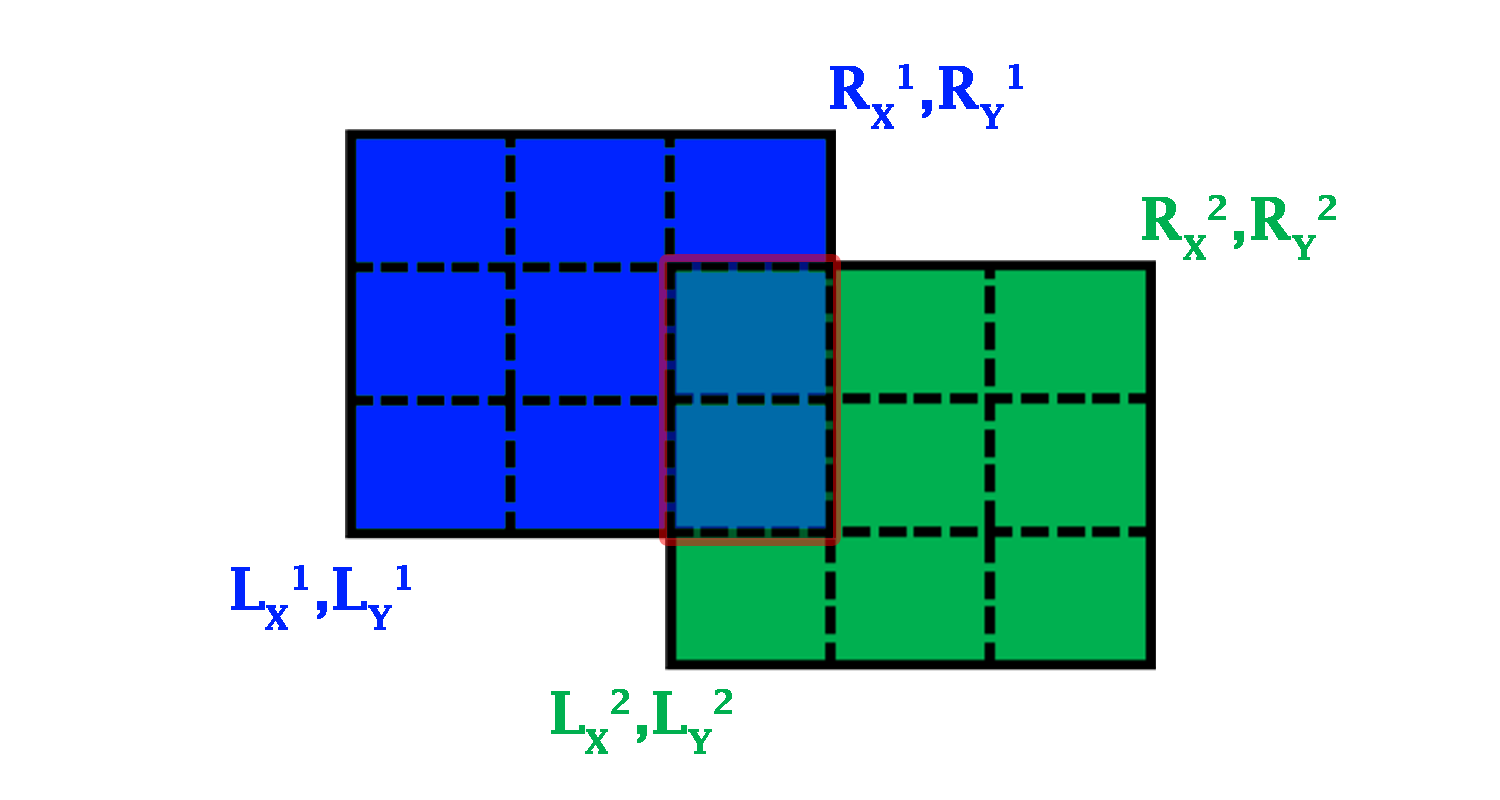
\includegraphics[width=\textwidth]{overlaps}
		\caption{Overlapping Model}
		\label{fig:overlaps}
	\end{figure}
	
	\item[] \textbf{Additional Constraints}
	\item[] In addition to the previous constraints, which are inevitable for the correct definition of the problem, we have decided to implement further constraints to restrict the domain of possible solutions and make the solver more efficient.
	\item \textbf{\textit{The total area of the presents must be the same of the Paper Sheet:}}
	\begin{itemize}
		\item[] $\sum_{i = 1}^{Presents}{Areas[i]} = Area$
		\item[] Thanks to this constraint we can understand from the beginning of the search if the given instance is feasible or not: in this way we can avoid the search a priori and avoid a waste of resources in case of unfeasibility.	
		\item[] A further relaxation of this constraint is to use $\leq$ instead of $=$ in order 
		to keep instances where we have presents that do not completely fill the Paper Sheet.  
		We kept the strict constraint for efficency reason, because the given instances all fall
		in this case.
	\end{itemize}
	\item \textbf{\textit{The presents must fill the row (column) dimension:}}
	\begin{itemize}
		\item[] A further step to optimize our solver was to add a constraint where it is checked whether each row \textit{(column)} is filled completely along its width \textit{(height)}.
		\item[] Here follow the two different definitions of this constraint:
		\item[] Rows: $
		\forall y \in [1, Height] \rightarrow\\ \sum_{i = 1}^{Presents}{
			\begin{cases}
				Dimension_x[i] & \text{if } y \geq Coord_y[i] \wedge y < Coord_y[i] + Dimension_y[i] \\
				0 & \text{otherwise}
			\end{cases}
		}\\= Width$
		\item[] Columns: $
		\forall x \in [1, Width] \rightarrow\\ \sum_{i = 1}^{Presents}{
			\begin{cases}
				Dimension_y[i] & \text{if } x \geq Coord_x[i] \wedge x < Coord_x[i] + Dimension_x[i] \\
				0 & \text{otherwise}
			\end{cases}
		}\\= Height$
	\end{itemize}
\end{itemize}


\begin{center}
    \begin{tabular}{|c|c|r|r|}
        \hline
        \multicolumn{4}{|c|}{\textbf{Results}} \\
        \hline
        \textbf{Instance} & \textbf{Time} & \textbf{Nodes} & \textbf{Propagations} \\
        
        \hline
		8x8 & 00:00:00.024 & 7 & 196 \\ \hline
		9x9 & 00:00:00.024 & 15 & 335 \\ \hline
		10x10 & 00:00:00.018 & 44 & 954 \\ \hline
		11x11 & 00:00:00.040 & 148 & 5,707 \\ \hline
		12x12 & 00:00:00.039 & 214 & 5,214 \\ \hline
		13x13 & 00:00:00.041 & 54 & 1,119 \\ \hline
		14x14 & 00:00:00.043 & 96 & 2,641 \\ \hline
		15x15 & 00:00:00.066 & 507 & 5,574 \\ \hline
		16x16 & 00:00:00.105 & 388 & 22,306 \\ \hline
		17x17 & 00:00:00.193 & 781 & 40,421 \\ \hline
		18x18 & 00:00:00.984 & 5,922 & 449,119 \\ \hline
		19x19 & 00:00:00.443 & 3,356 & 143,315 \\ \hline
		20x20 & 00:00:00.504 & 2,378 & 199,929 \\ \hline
		21x21 & 00:00:00.729 & 5,095 & 348,298 \\ \hline
		22x22 & 00:00:00.446 & 3,668 & 209,723 \\ \hline
		23x23 & 00:00:00.984 & 7,436 & 439,412 \\ \hline
		24x24 & 00:00:01.172 & 7,531 & 527,852 \\ \hline
		25x25 & 00:00:02.296 & 10,267 & 906,606 \\ \hline
		26x26 & 00:00:18.432 & 23,295 & 2,385,900 \\ \hline
		27x27 & 00:00:03.940 & 14,291 & 1,122,428 \\ \hline
		28x28 & 00:00:37.466 & 32,367 & 5,398,044 \\ \hline
		29x29 & 00:00:44.512 & 48,695 & 7,833,701 \\ \hline
		30x30 & 00:00:06.008 & 6,134 & 452,326 \\ \hline
		31x31 & 00:00:01.404 & 5,586 & 477,150 \\ \hline
		32x32 & 00:02:12.063 & 124,685 & 28,828,494 \\ \hline
		33x33 & 00:00:34.455 & 34,530 & 4,603,388 \\ \hline
		34x34 & 00:00:07.254 & 10,249 & 925,691 \\ \hline
		35x35 & 00:00:24.671 & 28,195 & 3,962,940 \\ \hline
		36x36 & 00:00:27.781 & 11,203 & 1,273,816 \\ \hline
		37x37 & 00:05:05.860 & 198,820 & 62,031,017 \\ \hline
		38x38 & 00:00:03.388 & 7,515 & 1,216,248 \\ \hline
		39x39 & 00:03:12.324 & 172,697 & 45,713,826 \\ \hline
		40x40 & 00:00:02.630 & 6,383 & 859,687 \\ \hline
		rotation\_test & - & - & - \\ \hline

    \end{tabular}
\end{center}


\section{Symmmetry Model}
As has already been done for the implementation in CP, also here we have decided to apply a similar method of \textbf{symmetry breaking} to remove rotated or mirrored solutions. To do this we used the heuristic to select the most voluminous presents (in this case we intend those with the largest area) first and place them in the lowest-left available place \cite{binpack, algdesign}. This allows us to always work in the lower left quadrant so as to avoid specular solutions that differ only from the reference quadrant. \\
As in the analogous model for CP, here too we have extracted the \textit{``Sorted Area Indexes"} parameter, which is essential to implement the heuristics just described:

\begin{center}
	\begin{adjustwidth}{-1.5cm}{}
		\begin{tabular}{|c|c|c|}
			\hline
			\multicolumn{3}{|c|}{\textbf{Extracted Parameters}} \\
			\hline
			\textbf{Parameter} & \textbf{Formula} & \textbf{Description} \\
			\hline
			Sorted Areas Indexes & \makecell{$Sorted\_Areas\_Indexes =$ \\ $reverse(arg\_sort(Areas))$} & Indexes of the Areas sorted by Present Area \\
			\hline
		\end{tabular}
	\end{adjustwidth}
\end{center}

In the \textit{``Sorted Area Indexes"} parameter, as can be seen from the name, is a list with the indices of the gifts arranged in ascending order with respect to the area.
In this way we can easily define that the first object of the list should be placed first in the lower-left corner of our paper in a hard-coded way:\\ \\
$
Coord\_X[Sorted\_Areas\_Indexes[1]] = 1\\
Coord\_Y[Sorted\_Areas\_Indexes[1]] = 1
$
\\ \\
In the same way we can go have all of the following presents in the list in order to respect the rule ``the biggest first":\\ \\
$
\forall i, j \in [1, Presents], j > i \rightarrow \\
Coord_y[Sorted\_Areas_Indexes[i]] = Coord_y[Sorted\_Areas\_Indexes[j]] \rightarrow \\
Coord_x[Sorted\_Areas_Indexes[i]] < Coord_x[Sorted\_Areas\_Indexes[j]]
$
\\

% TODO: Example Image


\begin{center}
    \begin{tabular}{|c|c|r|r|r|}
        \hline
        \multicolumn{5}{|c|}{\textbf{Results - SMT - Symmetry Model}} \\
        \hline
        \textbf{Instance} & \textbf{Time} & \textbf{Nodes} & \textbf{Propagations} & \textbf{Memory \textit{[KB]}} \\
        
        \hline
		8x8 & 00:00:00.021 & 52 & 140 & 211,940 \\ \hline
		9x9 & 00:00:00.019 & 103 & 471 & 211,940 \\ \hline
		10x10 & 00:00:00.021 & 374 & 607 & 87,820 \\ \hline
		11x11 & 00:00:00.041 & 142 & 2,295 & 87,820 \\ \hline
		12x12 & 00:00:00.084 & 487 & 17,402 & 87,820 \\ \hline
		13x13 & 00:00:00.095 & 257 & 26,864 & 87,820 \\ \hline
		14x14 & 00:00:00.100 & 362 & 21,240 & 87,820 \\ \hline
		15x15 & 00:00:00.159 & 525 & 57,603 & 87,820 \\ \hline
		16x16 & 00:00:00.087 & 399 & 12,846 & 87,820 \\ \hline
		17x17 & 00:00:00.371 & 1,088 & 165,078 & 87,820 \\ \hline
		18x18 & 00:00:25.060 & 20,254 & 4,655,919 & 87,820 \\ \hline
		19x19 & 00:00:01.458 & 3,160 & 684,733 & 87,820 \\ \hline
		20x20 & 00:00:00.651 & 3,022 & 313,670 & 87,820 \\ \hline
		21x21 & 00:00:01.386 & 4,354 & 629,898 & 87,820 \\ \hline
		22x22 & 00:00:00.371 & 1,802 & 98,081 & 87,820 \\ \hline
		23x23 & 00:00:23.778 & 17,883 & 3,802,390 & 87,820 \\ \hline
		24x24 & 00:00:03.223 & 9,188 & 969,847 & 87,820 \\ \hline
		25x25 & 00:00:08.041 & 6,649 & 1,113,972 & 87,820 \\ \hline
		26x26 & 00:00:24.968 & 22,894 & 4,452,757 & 130,759 \\ \hline
		27x27 & 00:00:10.064 & 14,148 & 2,083,453 & 87,820 \\ \hline
		28x28 & 00:00:08.320 & 9,009 & 1,132,277 & 87,820 \\ \hline
		29x29 & 00:00:33.789 & 24,402 & 3,906,977 & 88,600 \\ \hline
		30x30 & 00:00:13.749 & 13,058 & 1,021,942 & 130,759 \\ \hline
		31x31 & 00:00:11.827 & 4,628 & 500,544 & 130,759 \\ \hline
		32x32 & 00:05:20.900 & 162,248 & 72,507,269 & 228,930 \\ \hline
		33x33 & 00:00:57.685 & 48,708 & 13,329,045 & 88,770 \\ \hline
		34x34 & 00:00:15.569 & 12,762 & 1,623,818 & 88,770 \\ \hline
		35x35 & 00:00:24.271 & 21,457 & 3,966,717 & 189,550 \\ \hline
		36x36 & 00:00:42.454 & 30,754 & 7,084,316 & 91,320 \\ \hline
		37x37 & 00:02:58.149 & 121,821 & 38,672,489 & 189,550 \\ \hline
		38x38 & 00:00:19.120 & 17,460 & 2,821,474 & 91,320 \\ \hline
		39x39 & 00:09:31.279 & 202,553 & 55,241,230 & 193,430 \\ \hline
		40x40 & 00:00:08.420 & 11,007 & 1,357,752 & 211,940 \\ \hline
		rotation\_test & - & - & - & - \\ \hline

    \end{tabular}
\end{center}



\section{Rotation Model}
In order to expand our model so that it is possible to rotate a block, thus having further solutions to explore in our problem, we needed to add a new \textit{``rotated"} variable:
\begin{center}
		\begin{tabular}{|c|c|}
			\hline
			\multicolumn{2}{|c|}{\textbf{Variables}} \\
			\hline
			\textbf{Variable} & {\textbf{Description}} \\
			\hline
			Rotated & The boolean array that indicates whether a present is rotated or not \\
			\hline
		\end{tabular}
\end{center}
If \textit{``rotated"} were set to True, the dimensions X and Y would be swapped to represent the present rotated by 90 ° (or 270 °). In the False case, the dimensions remain unchanged and represent the object not rotated (or rotated by 180 °). \\
All this is easily implemented with a boolean check when returning the dimensions of a single present.
Here follows the definition of what just described:\\
$
Get\_Dimension_x = 
\begin{cases}
	Dimension_y & \text{if } Rotated \\
	Dimension_x & \text{otherwise}
\end{cases}
$
\\
$
Get\_Dimension_y = 
\begin{cases}
	Dimension_x & \text{if } Rotated \\
	Dimension_y & \text{otherwise}
\end{cases}
$


\begin{center}
    \begin{tabular}{|c|c|r|r|r|}
        \hline
        \multicolumn{5}{|c|}{\textbf{Results}} \\
        \hline
        \textbf{Instance} & \textbf{Time} & \textbf{Nodes} & \textbf{Propagations} & \textbf{Memory} \\
        
        \hline
		8x8 & - & - & - & - \\ \hline
		9x9 & - & - & - & - \\ \hline
		10x10 & 00:00:00.144 & 721 & 26,685 & 211,940 \\ \hline
		11x11 & 00:00:00.067 & 579 & 5,680 & 211,940 \\ \hline
		12x12 & 00:00:01.408 & 5,214 & 443,395 & 211,940 \\ \hline
		13x13 & 00:00:00.448 & 2,119 & 140,276 & 211,940 \\ \hline
		14x14 & 00:00:02.592 & 8,111 & 756,747 & 211,940 \\ \hline
		15x15 & 00:00:02.032 & 7,798 & 683,163 & 211,940 \\ \hline
		16x16 & 00:00:03.967 & 11,880 & 1,238,221 & 211,940 \\ \hline
		17x17 & 00:00:26.176 & 5,651 & 364,315 & 211,940 \\ \hline
		18x18 & 00:00:28.966 & 18,584 & 1,035,514 & 211,940 \\ \hline
		19x19 & 00:00:32.796 & 22,376 & 2,354,741 & 211,940 \\ \hline
		20x20 & 00:00:29.592 & 16,027 & 1,459,495 & 211,940 \\ \hline
		21x21 & 00:00:46.402 & 39,691 & 8,637,344 & 189,550 \\ \hline
		22x22 & 00:00:35.597 & 25,020 & 3,011,708 & 211,940 \\ \hline
		23x23 & 00:00:36.571 & 37,053 & 2,927,184 & 189,550 \\ \hline
		24x24 & 00:01:18.530 & 83,289 & 15,993,390 & 228,930 \\ \hline
		25x25 & 00:02:36.290 & 140,045 & 25,825,689 & 211,940 \\ \hline
		26x26 & 00:05:18.520 & 266,107 & 58,347,287 & 189,550 \\ \hline
		27x27 & 00:04:49.714 & 248,500 & 62,248,419 & 228,930 \\ \hline
		28x28 & 00:03:14.506 & 175,627 & 37,562,461 & 127,420 \\ \hline
		29x29 & 00:18:32.908 & 564,825 & 144,571,773 & 320,540 \\ \hline
		30x30 & 00:02:23.401 & 141,093 & 29,682,469 & 228,930 \\ \hline
		31x31 & 00:00:53.787 & 55,579 & 7,421,610 & 228,930 \\ \hline
		32x32 & - & - & - & - \\ \hline
		33x33 & 00:04:09.668 & 218,937 & 46,436,633 & 320,540 \\ \hline
		34x34 & 00:00:36.893 & 24,340 & 4,007,587 & 320,540 \\ \hline
		35x35 & 00:03:51.419 & 182,898 & 42,674,674 & 320,540 \\ \hline
		36x36 & 00:05:13.999 & 222,110 & 57,051,458 & 320,540 \\ \hline
		37x37 & - & - & - & - \\ \hline
		38x38 & - & - & - & - \\ \hline
		39x39 & - & - & - & - \\ \hline
		40x40 & - & - & - & - \\ \hline
		rotation\_test & - & - & - & - \\ \hline

    \end{tabular}
\end{center}


\section{Symmetry Rotation Model}
Following as done in CP, also in SMT we decided to combine the characteristics of the previously implemented models.\\
We merge together the \textbf{Symmetry Model} with the \textbf{Rotation Model} and we made
the \textbf{Symmetry Rotation Model} that takes in account the possibility of the presents rotation and also excludes the symmetrical
solutions.


\begin{center}
    \begin{tabular}{|c|c|r|r|}
        \hline
        \multicolumn{4}{|c|}{\textbf{Results}} \\
        \hline
        \textbf{Instance} & \textbf{Time} & \textbf{Nodes} & \textbf{Propagations} \\
        
        \hline
		8x8 & - & - & - \\ \hline
		9x9 & - & - & - \\ \hline
		10x10 & - & - & - \\ \hline
		11x11 & - & - & - \\ \hline
		12x12 & - & - & - \\ \hline
		13x13 & - & - & - \\ \hline
		14x14 & - & - & - \\ \hline
		15x15 & - & - & - \\ \hline
		16x16 & - & - & - \\ \hline
		17x17 & - & - & - \\ \hline
		18x18 & - & - & - \\ \hline
		19x19 & - & - & - \\ \hline
		20x20 & - & - & - \\ \hline
		21x21 & - & - & - \\ \hline
		22x22 & - & - & - \\ \hline
		23x23 & - & - & - \\ \hline
		24x24 & - & - & - \\ \hline
		25x25 & - & - & - \\ \hline
		26x26 & - & - & - \\ \hline
		27x27 & - & - & - \\ \hline
		28x28 & - & - & - \\ \hline
		29x29 & - & - & - \\ \hline
		30x30 & - & - & - \\ \hline
		31x31 & - & - & - \\ \hline
		32x32 & - & - & - \\ \hline
		33x33 & - & - & - \\ \hline
		34x34 & - & - & - \\ \hline
		35x35 & - & - & - \\ \hline
		36x36 & - & - & - \\ \hline
		37x37 & - & - & - \\ \hline
		38x38 & - & - & - \\ \hline
		39x39 & - & - & - \\ \hline
		40x40 & - & - & - \\ \hline
		rotation\_test & - & - & - \\ \hline

    \end{tabular}
\end{center}



\section{Duplicated Symmetry Model}
As we did in the CP models, we can model those instances that have presents with the same dimensions. As we modelled the problem,
the \textbf{Base Model} can already solve this kind of instances, but we can add some constraints to take in account symmterical solutions.
The simpliest approach is to force the same size presents to be placed in the order they appear. In this way we put in the lesser
coordinates the presents that are in the first positions of the parameter $Dimension_X$ and $Dimension_y$ arrays:\\

$
\forall i, j \in [1, Presents], j > i \rightarrow \\
    Dimension_x[Sorted\_Areas\_Indexes[i]] \neq Dimension_x[Sorted\_Areas\_Indexes[j]] \wedge \\
    Dimension_y[Sorted\_Areas\_Indexes[i]] \neq Dimension_y[Sorted\_Areas\_Indexes[j]] \wedge \\
    Coord_y[Sorted\_Areas\_Indexes[i]] \leq Coord_y[Sorted\_Areas\_Indexes[j]]
$

By adding this constraint, we force the solver to exclude the solutions where the same size presents can swap each other,
just by forcing the solver to put them in the lesser coordinates possible as before they appear in the parameter dimensions array.


\begin{center}
    \begin{tabular}{|c|c|r|r|}
        \hline
        \multicolumn{4}{|c|}{\textbf{Results}} \\
        \hline
        \textbf{Instance} & \textbf{Time} & \textbf{Nodes} & \textbf{Propagations} \\
        
        \hline
		8x8 & - & - & - \\ \hline
		9x9 & - & - & - \\ \hline
		10x10 & - & - & - \\ \hline
		11x11 & - & - & - \\ \hline
		12x12 & - & - & - \\ \hline
		13x13 & - & - & - \\ \hline
		14x14 & - & - & - \\ \hline
		15x15 & - & - & - \\ \hline
		16x16 & - & - & - \\ \hline
		17x17 & - & - & - \\ \hline
		18x18 & - & - & - \\ \hline
		19x19 & - & - & - \\ \hline
		20x20 & - & - & - \\ \hline
		21x21 & - & - & - \\ \hline
		22x22 & - & - & - \\ \hline
		23x23 & - & - & - \\ \hline
		24x24 & - & - & - \\ \hline
		25x25 & - & - & - \\ \hline
		26x26 & - & - & - \\ \hline
		27x27 & - & - & - \\ \hline
		28x28 & - & - & - \\ \hline
		29x29 & - & - & - \\ \hline
		30x30 & - & - & - \\ \hline
		31x31 & - & - & - \\ \hline
		32x32 & - & - & - \\ \hline
		33x33 & - & - & - \\ \hline
		34x34 & - & - & - \\ \hline
		35x35 & - & - & - \\ \hline
		36x36 & - & - & - \\ \hline
		37x37 & - & - & - \\ \hline
		38x38 & - & - & - \\ \hline
		39x39 & - & - & - \\ \hline
		40x40 & - & - & - \\ \hline
		rotation\_test & - & - & - \\ \hline

    \end{tabular}
\end{center}


\section{Duplicated Symmetry Rotation Model}

This model simply incorporates all the features implemented in the previous models \textit{(Symmetry, Rotation, Duplicated Presents)}.
\\
In this way it is possible to benefit at the same time from features, such as rotation and the distinction between two different gifts of the same size, and from symmetry breaking to remove rotated and mirrored solutions from the domain.  



\begin{center}
    \begin{tabular}{|c|c|r|r|}
        \hline
        \multicolumn{4}{|c|}{\textbf{Results}} \\
        \hline
        \textbf{Instance} & \textbf{Time} & \textbf{Nodes} & \textbf{Propagations} \\
        
        \hline
		8x8 & - & - & - \\ \hline
		9x9 & - & - & - \\ \hline
		10x10 & - & - & - \\ \hline
		11x11 & - & - & - \\ \hline
		12x12 & - & - & - \\ \hline
		13x13 & - & - & - \\ \hline
		14x14 & - & - & - \\ \hline
		15x15 & - & - & - \\ \hline
		16x16 & - & - & - \\ \hline
		17x17 & - & - & - \\ \hline
		18x18 & - & - & - \\ \hline
		19x19 & - & - & - \\ \hline
		20x20 & - & - & - \\ \hline
		21x21 & - & - & - \\ \hline
		22x22 & - & - & - \\ \hline
		23x23 & - & - & - \\ \hline
		24x24 & - & - & - \\ \hline
		25x25 & - & - & - \\ \hline
		26x26 & - & - & - \\ \hline
		27x27 & - & - & - \\ \hline
		28x28 & - & - & - \\ \hline
		29x29 & - & - & - \\ \hline
		30x30 & - & - & - \\ \hline
		31x31 & - & - & - \\ \hline
		32x32 & - & - & - \\ \hline
		33x33 & - & - & - \\ \hline
		34x34 & - & - & - \\ \hline
		35x35 & - & - & - \\ \hline
		36x36 & - & - & - \\ \hline
		37x37 & - & - & - \\ \hline
		38x38 & - & - & - \\ \hline
		39x39 & - & - & - \\ \hline
		40x40 & - & - & - \\ \hline
		rotation\_test & - & - & - \\ \hline

    \end{tabular}
\end{center}


\section{Remarks and Results}
We briefly recap the overall results of the previous models in a textual informative table:

\begin{center}
    \begin{tabular}{|c|c|c|c|c|}
        \hline
        \multicolumn{5}{|c|}{\textbf{Global Results}} \\
        \hline
        \textbf{Model} & \textbf{Speed} & \textbf{Complexity} & \textbf{Strengths} & \textbf{Weaknesses} \\
        \hline
    \end{tabular}
\end{center}